\NewDocumentCommand{\EId}{}{%

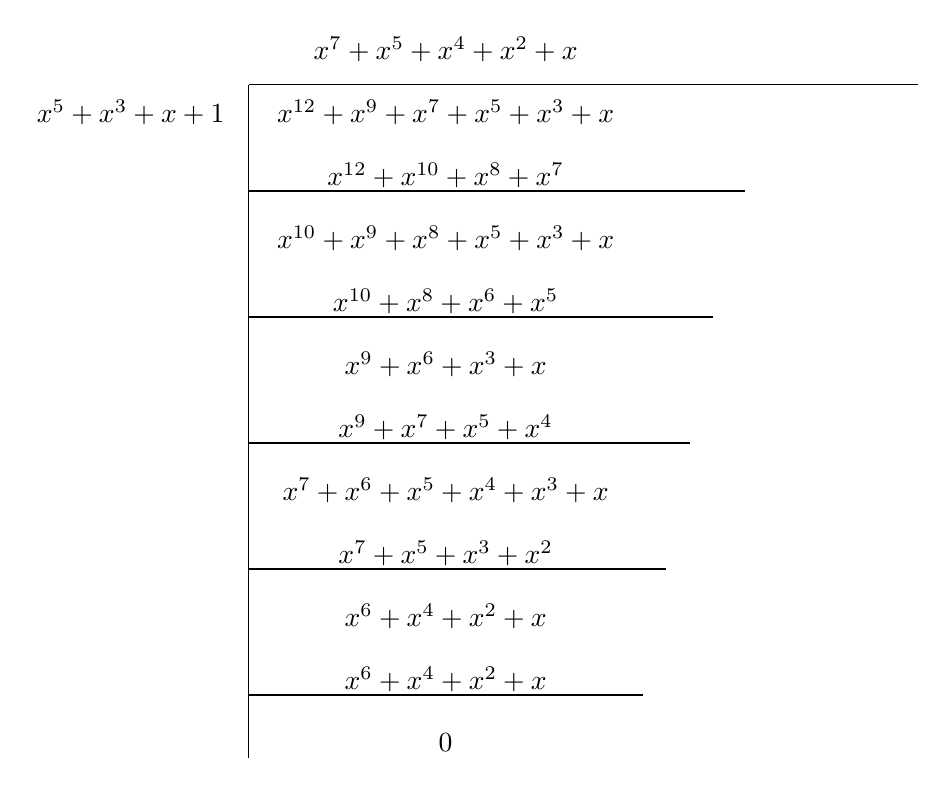
\begin{tikzpicture}[font=\normalsize]

% Coordinates are now the center of each node
% and all rows share the same x-coordinate

% Dividend
\node (A) at (2,0)
{$x^{12}+x^9+x^7+x^5+x^3+x$};

% Divisor
\node at (-2,0)
{$x^5+x^3+x+1$};

% Division symbol
\draw (-0.5,0.35)--(-0.5,-8.2);
\draw (-0.5,0.35)--(8,0.35);

% Quotient
\node at (2,0.8)
{$x^7+x^5+x^4+x^2+x$};

% Step 1
\node at (2,-0.8)
{$x^{12}+x^{10}+x^8+x^7$};

\draw (-.5,-1.0)--(5.8,-1.0);

\node at (2,-1.6)
{$x^{10}+x^9+x^8+x^5+x^3+x$};

% Step 2
\node at (2,-2.4)
{$x^{10}+x^8+x^6+x^5$};

\draw (-.5,-2.6)--(5.4,-2.6);

\node at (2,-3.2)
{$x^9+x^6+x^3+x$};

% Step 3
\node at (2,-4.0)
{$x^9+x^7+x^5+x^4$};

\draw (-.5,-4.2)--(5.1,-4.2);

\node at (2,-4.8)
{$x^7+x^6+x^5+x^4+x^3+x$};

% Step 4
\node at (2,-5.6)
{$x^7+x^5+x^3+x^2$};

\draw (-.5,-5.8)--(4.8,-5.8);

\node at (2,-6.4)
{$x^6+x^4+x^2+x$};

% Step 5
\node at (2,-7.2)
{$x^6+x^4+x^2+x$};

\draw (-.5,-7.4)--(4.5,-7.4);

\node at (2,-8.0)
{$0$};

\end{tikzpicture}
}

\NewDocumentCommand{\EIIa}{}{%
\begin{tikzpicture}[font=\small]
% Dividend
\node (A) at (2,0)
{$x^6+x^5+x^3+x^2+1$};

% Divisor
\node at (-2,0)
{$x^3+x+1$};

% Division bracket
\draw (-0.5,0.35)--(-0.5,-6.8);
\draw (-0.5,0.35)--(7,0.35);

% Quotient
\node at (2,0.8)
{$x^3+x^2+x+1$};

% Step 1
\node at (2,-0.8)
{$x^6+x^4+x^3$};

\draw (-.5,-1.0)--(4.8,-1.0);

\node at (2,-1.6)
{$x^5+x^4+x^2+1$};


% Step 2
\node at (2,-2.4)
{$x^5+x^3+x^2$};

\draw (-.5,-2.6)--(4.5,-2.6);

\node at (2,-3.2)
{$x^4+x^3+1$};


% Step 3
\node at (2,-4.0)
{$x^4+x^2+x$};

\draw (-.5,-4.2)--(4.3,-4.2);

\node at (2,-4.8)
{$x^3+x^2+x+1$};


% Step 4
\node at (2,-5.6)
{$x^3+x+1$};

\draw (-.5,-5.8)--(4.0,-5.8);

\node at (2,-6.4)
{$x^2$};
\end{tikzpicture}

}

\NewDocumentCommand{\EIIIb}{}{%
\begin{tikzpicture}[font=\small]

% Dividend
\node (A) at (2,0)
{$x^4+x^3+1$};

% Divisor
\node at (-2,0)
{$x^2+x+1$};

% Division bracket
\draw (-0.5,0.35)--(-0.5,-4);
\draw (-0.5,0.35)--(5.5,0.35);

% Quotient
\node at (2,0.8)
{$x^2+1$};

%--------------------------------------------------
% Step 1
%--------------------------------------------------
\node at (2,-0.8)
{$x^4+x^3+x^2$};

\draw (-.5,-1.0)--(4.3,-1.0);

\node at (2,-1.6)
{$x^2+1$};

%--------------------------------------------------
% Step 2
%--------------------------------------------------
\node at (2,-2.4)
{$x^2+x+1$};

\draw (-.5,-2.6)--(3.8,-2.6);

\node at (2,-3.2)
{$x$};

\end{tikzpicture}

}

\NewDocumentCommand{\EVa}{}{%
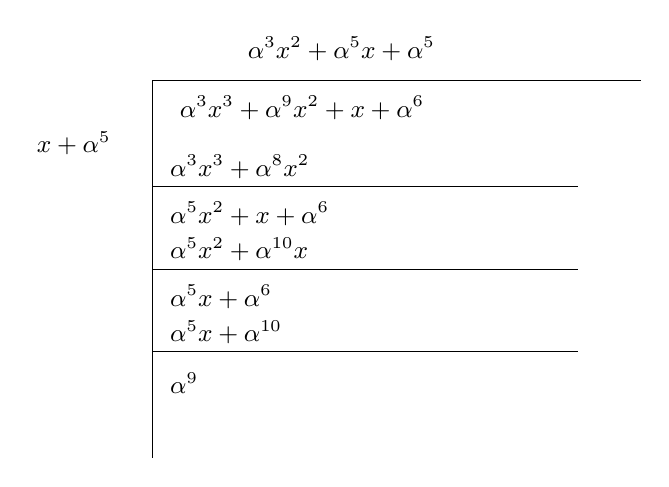
\begin{tikzpicture}[font=\small]

% Quotient
\node at (4.2,1.2)
{$\alpha^3x^2+\alpha^5x+\alpha^5$};

% Main division bracket
\draw (1.8,0.8) -- (1.8,-4.0);
\draw (1.8,0.8) -- (8.0,0.8);

% Divisor
\node at (0.8,0.0)
{$x+\alpha^5$};

% Dividend
\node at (3.7,0.45)
{$\alpha^3x^3+\alpha^9x^2+x+\alpha^6$};


% First addition step
\node[anchor=west] at (1.9,-0.3)
{$\alpha^3x^3+\alpha^8x^2$};

\draw (1.8,-0.55) -- (7.2,-0.55);

\node[anchor=west] at (1.9,-0.9)
{$\alpha^5x^2+x+\alpha^6$};


% Second addition step
\node[anchor=west] at (1.9,-1.35)
{$\alpha^5x^2+\alpha^{10}x$};

\draw (1.8,-1.6) -- (7.2,-1.6);

\node[anchor=west] at (1.9,-1.95)
{$\alpha^5x+\alpha^6$};


% Third addition step
\node[anchor=west] at (1.9,-2.4)
{$\alpha^5x+\alpha^{10}$};

\draw (1.8,-2.65) -- (7.2,-2.65);

% Remainder
\node[anchor=west] at (1.9,-3.05)
{$\alpha^9$};

\end{tikzpicture}
}